\section{Обзор существующих решений}
\label{sec:Section2} \index{Section2}

\subsection{Формат сигнатур}

Прежде чем говорить непосредственно о методах автоматической генерации сигнатур, стоит сначала понять, какие бывают сигнатуры и в каком формате они могут быть представлены.

Существует несколько представлений сигнатур. Некоторые из этих видов использовались для представлений сигнатур червей.
В работе \cite{newsome2005polygraph} приводится следующая классификация:

\begin{itemize}
    \item \textbf{Конъюнктивная сигнатура}: cостоит из набора подстрок (или токенов), полезная нагрузка соотвествует ей, если все токены в наборе были найдены в любом порядке.
    \item \textbf{Сигнатура, представленная последовательностью токенов}: состоит из упорядоченного набора токенов.
    Полезная нагрузка соотвествует сигнатуре, если она содержит всю последовательность токенов в том же порядке.
    \item \textbf{Байесовская сигнатура}: состоит из набора токенов, каждый из которых связан с оценкой, и общего порогового значения.
    Байесовские сигнатуры обеспечивают вероятностное сопоставление: вычисляется вероятность сопоставления, используя оценки присутствующих токенов в полезной нагрузки.
    Если результирующая вероятность превышает пороговое значение, то считается, что полезная нагрузка совпала с сигнатурой.
\end{itemize}

При использовании любого из этих определений в качестве определения сигнатуры приложения/протокола возникают некоторые специфические проблемы:

\begin{enumerate}
    \item \textbf{Разнообразие протоколов приложения}: два потока, принадлежащие одному и тому же приложению, могут иметь разные общие подстроки.
    Например, приложения P2P используют разные протоколы для обмена одноранговой информацией и данными. Кроме того приложения будут обновлять свои протоколы.
    Потоки различных версий протоколов могут существовать в сети одновременно.
    Ни конъюктивная сигнатура, ни сигнатура, представленная токен-подпоследовательностью, не могут выражать несколько протоколов.
    \item \textbf{Взаимоисключающее свойство некоторых подстрок в прикладных протоколах}.
    Например, протокол Gnutella имеет две последовательности подстрок $\{$'Get' 'UserAgent'$\}$ и $\{$'HTTP' 'User-Agent'$\}$.
    Подстроки 'Get' и 'HTTP' не будут отображаться в одном и том же потоке в протоколе Gnutella.
    Две общие подстроки являются взаимоисключающими, но байесовские сигнатуры не могут выражать взаимоисключающее свойство.
\end{enumerate}

Определение сигнатуры, основанное на регулярных выражениях, становится очень распространнённым в классификации приложений \cite{szabo2012automatic, wang2012generating, vinothgeorge2013efficient}.
Однако процесс сопоставления регулярных выражений требует огромной вычислительной мощности,
которая слабо масштабируется для идентификации сетевого трафика в режиме реального времени.
Способ построения регулярного выражения оказывает непосредственное влияние на классификацию потоков и на общую производительность сопоставления.
Несмотря на это, некоторые системы DPI используют регулярные выражения для представления сигнатур приложений.
Система обнаружения/предотвращения вторжений Snort (IDS/IPS) \cite{Snort}
имеет множество сигнатур приложений и предлагает пользователю возможность вставлять новые регулярные выражения по требованию.

Почти неизвестно алгоритмов извлечения сигнатур в виде регулярных выражений, а те что есть -
основаны на строках и небольшом подмножестве операций, которые есть в регулярных выражениях.
Поэтому дальше будем рассматривать сигнатуры только в виде строк.

Среди возможных описаний строковых сигнатур, набор последовательностей подстрок является наилучшим определением сигнатуры.
Полезная нагрузка соотвествует сигнатуре, если она содержит какую-то последовательность подстрок из этого набора. Такое определение решает описанные выше проблемы.

Введем следующее определение: уровень поддержки последовательности подстрок (support) равен отношению количества хостов, использующих соответствующее приложение или протокол и
трафик которого содержит эту последовательность подстрок к общему количеству хостов, использующих соответствующее приложение или протокол.

При заданном формате, в общем случае, не любая последовательность подстрок из набора охватывает все хосты.
В части из дальнейших рассматриваемых методов считается, что сигнатура состоит из одной последовательности подстрок, уровень поддержки которой равен 1,
то есть она присутствует в трафике каждого хоста, использующего рассматриваемый протокол или приложение.
Этот показатель можно использовать как параметр в некоторых из этих методов.

\subsection{Структура сигнатур}

Большинство форматов сигнатур в предыдущих работах \cite{park2008towards,ye2009autosig,santosautomatic} представляют собой простые подстроки, которые часто появляются в полезной нагрузке.
Следовательно, всё ещё существует вероятность того, что извлеченные сигнатуры полезной нагрузки могут быть не специфичными для конкретного приложения,
некоторые могут принадлежать и другому приложению. Это называется избыточностью сигнатур.

Для улучшения качества сигнатур предлагается выделить три типа сигнатур \cite{goo2016payload, shim2019automatic}:

\begin{enumerate}
    \item сигнатура содержимого (полезной нагрузки),
    \item сигнатура пакета,
    \item сигнатура потока.
\end{enumerate}

\begin{figure}[h!]
    \begin{center}
        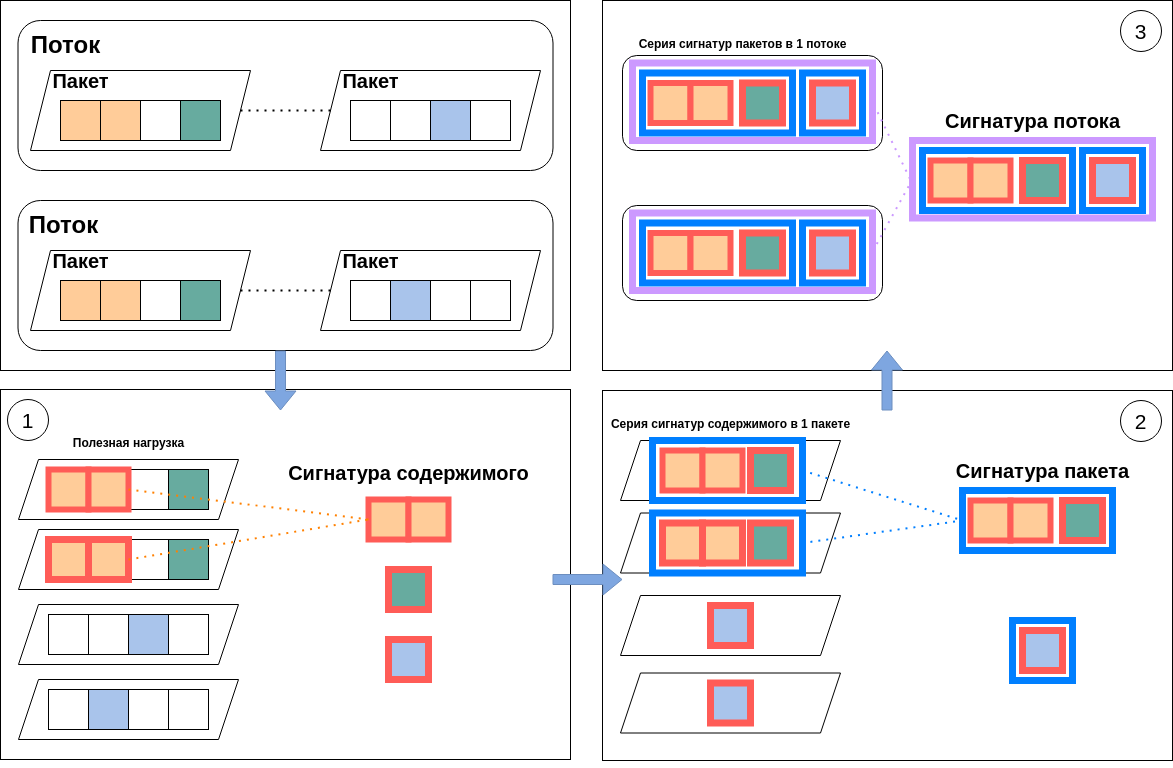
\includegraphics[width = \textwidth]{signature_structure.png}
        \caption{Процесс извлечения предлагаемой структуры сигнатур полезной нагрузки.}\label{signature_process}
    \end{center}
\end{figure}

Сигнатура содержимого определяется как различимая и уникальная подстрока полезной нагрузки, состоящая из непрерывных символов или шестнадцатеричных значений.
На самом деле уникальность с помощью одной подстроки тяжело обеспечить, например, такие строки ``GET''  или ``HTTP'', которые часто встречаются в HTTP,
не могут служить конечными сигнатурами, так как они не различают приложения.

Сигнатура пакета состоит из серии сигнатур содержимого, которые появляются в одном пакете.
Так как классификация может выполняться без накопления пакетов, то есть без сбора потока, то анализируется всегда хотя бы один пакет.
Это значит, что для классификации всегда можно использовать сигнатуры пакетов, и не имеет смысла использовать отдельно сигнатуры содержимого.

Сигнатура потока состоит из серии сигнатур пакетов, которые появляются в одном потоке, где под потоком понимается набор пакетов, имеющий одни и те же
IP-адрес источника, IP-адрес назначения, порт источника, порт назначения и используемый протокол транспортного уровня.
Сигнатура потока гораздо более специфична для конкретного приложения, чем сигнатура пакета, и значительно повышает точность.

Поэтапный процесс извлечения сигнатур представлен на рис. \ref{signature_process}. Как можно заметить, данная структура сигнатур обладает свойством вложенности.

\subsection{Метрики оценки качества сигнатур}

Для оценки качества получаемых сигнатур рассмотрим матрицу ошибок: 4 стандартные категории,
к котором можно отнести результат работы классификатора на полученной сигнатуре.
В нашем случае рассматриваемый класс это целевой протокол или приложение.
Под классификацией трафика будем понимать классификацию конкретного пакета или потока в зависимости от того, какой уровень сигнатур используется.

\begin{table}[H]
\centering
\resizebox{\columnwidth}{!}
{
    \begin{tabular}{|c|c|c|}
    \hline
                                                                                                  & Принадлежит классу (P) & Не принадлежит классу (N) \\ \hline
    \begin{tabular}[c]{@{}c@{}}Предсказана принадлежность\\ к классу (T)\end{tabular}             & TP                     & TN                        \\ \hline
    \begin{tabular}[c]{@{}c@{}}Предсказано отсутствие \\ принадлежности к классу (F)\end{tabular} & FP                     & FN                        \\ \hline
    \end{tabular}
}
\end{table}

\begin{itemize}
    \item истинно положительный (TP): указывает, что трафик правильно классифицирован, как относящийся к определенному классу.
    \item истинно отрицательный (TN): указывает, что трафик правильно классифицирован, как не относящийся к определенному классу.
    \item ложно положительный (FP): указывает, что трафик неправильно классифицирован, как относящийся к определенному классу.
    \item ложный отрицательный (FN): указывает, что трафик неправильно классифицирован, как не относящийся к определенному классу.
\end{itemize}

Наиболее часто используемые показатели для классификации трафика определяются следующим образом:

\begin{itemize}
    \item Accuracy (достоверность) - доля правильных классификаций.
    $$ accuracy = \dfrac{TP + TN}{TP + TN + FP + FN} $$

    \item Recall (полнота) - отношение верно классифицированного трафика определенному классу к общему числу трафика этого класса,
    то есть описывает способность сигнатуры обнаружить данный целевой протокол или приложение.
    $$ recall = \dfrac{TP}{TP + FN} $$

    \item Precision (точность) - доля верно классифицированного трафика среди всего трафика, который классификатор отнёс к этому классу.
    $$ precision = \cfrac{TP}{TP + FP} $$

    \item $F_1$-score ($F_1$-мера) - гармоническое среднее между точностью и полнотой.
     $$ \textit{$F_1$-score} = \dfrac{2 \times recall \times precision}{recall + precision} $$
    Метрика accuracy может терять свой смысл в задачах с сильно неравными классами.
    Напротив же recall и precision не зависят от соотношения классов и поэтому применимы в случае несбалансированных классов,
    что является правдой для сетевого трафика. Часто на практике возникает задача найти оптимальный баланс между precision
    и recall. Для этих целей подходит F-мера, которая достигает максимума при recall
    и precision равным 1, и стремится к минимуму, если хотя бы один из параметров стремится к нулю.


\end{itemize}

Для сигнатур полезно ещё ввести такое понятие как:

\begin{itemize}
    \item Redundancy (избыточность) опредялется как:
    $$ \textit{Redundancy} = \frac{\text{Объём трафика идентифицированный двумя и более сигнатурами}}{\text{Объём трафика идентифицированый набором сигнатур}}$$
    Redundancy имеет значение от 0 до 1, где 0 - наилучшее значение, которое указывает на то, что все сигнатуры набора классифицируют исключительно только свою часть трафика,
    то есть являются уникальными и незаменяемыми. Если redundancy близка к 1, то в наборе присутствует ненужные сигнатуры, которые идентифицируют перекрывающийся трафик.
    По мере увеличения количества сигнатур увеличиваются и накладные расходы системы, поэтому данное значение должно оставаться низким.
\end{itemize}

\subsection{Обзор существующих методов автоматической генерации сигнатур}

Рассмотрим несколько существующих методов автоматической генерации сигнатур и опишем основной принцип их работы.

\subsubsection{LASER}

В статье \cite{park2008towards} описан алгоритм LASER (Application Signature ExtRaction),
который основан на задаче поиска наиболее длинной общей подпоследовательности LCS (Longest common subsequence).
Данный алгоритм автоматически определяет достоверный шаблон в полезной нагрузке пакета без предварительного знания форматов протоколов, то есть генерирует сигнатуру пакета.
За шаг извлечения сигнатуры был принят алгоритм LCS, который ранее в основном использовался для сопоставления последовательностей ДНК в приложениях биоинформатики \cite{ning2006finding}.
Он был модифицирован под текущие задачи.

Вводятся ограничения на модификацию LCS:

\begin{itemize}
    \item \textbf{Количество пакетов в потоке}.
    Нет необходимости проводить проверку над всеми пакетами в наборе,
    потому что сигнатура существует в нескольких начальных пакетах потока.
    \item \textbf{Минимальная длина подстроки}. Стоимость сопоставления сигнатур пропорциональна их длинам.
    Сгенерированная сигнатура состоит из последовательности подстрок.
    Чтобы избежать каких-либо тривиальных сигнатур,
    минимальная граница длины подстроки должна рассматриваться как ограничение для модифицированного алгоритма LCS.
    Имея это ограничение длины, предотвращается включение однопозиционных и многопозиционных символов в последовательность общих строк,
    например символа '/' в HTTP пакетах.
    \item \textbf{Сравнение размера пакетов}. Это увеличивает вероятность нахождения надёжной сигнатуры,
    если пакеты сгруппированы по назначению (например, управляющий трафик или трафик загрузки) и характеристикам трафика.
    Одной из таких характеристик является размер пакета. Обьём данных при установлении соединения небольшой.
    Конкретная сигнатура существует только в первых пакетах.
    Поэтому сравнения небольших пакетов установки соединения и пакетов загрузки нежелательно для генерации надёжной сигнатуры.

\end{itemize}

Приведём сам алгоритм из статьи:

\begin{lstlisting}[language=PL/I, caption=Алгоритм LASER]
procedure Signature_Generation ()
    Flow_Pool {F1[]...Fx[]} <- Santized_packet_collector
    F1[] <- Iterate, packet dump for Flow 1
    F2[] <- Iterate, packet dump for Flow 2
    while i from 0 to packet_constraint do
        while j from 0 to packet_constraint do
            if |F1[i].packet_size - F2[j].packet_size| < threshold
            result_LCS <- LASER (F1[i], F1[j])
            LCS_Pool{} <- Append result_LCS, end if
        j++, end while
    i++, end while
    S <- select the longest from LCS_Pool
    while i from 0 to number of rest flows of Flow_Pool do
        Fi <- select one from the rest of Flow_Pool
        result_LCS <- LASER (S, Fi)
        S <- select the longest from result_LCS
    i++, end while
    return S

procedure LASER (PacketA[1...m], PacketB[1...n])
    PacketA [m...1] <- Reverse byte stream
    PacketB [n...1] <- Reverse byte stream
    Matrix [m][n]
    while i from 0 to m do
        while j from 0 to n do
            if i = 0 or j = 0, then Matrix[i][j] = 0;
            else if PacketA[i] = PacketB[j], then
                Matrix [i][j] <- 'Diagonal',
                Matrix [i][j] = Matrix [i-1][j-1] + 1;
            else if Matrix[i-1][j] >= Matrix[i][j-1], then
                Matrix[i][j] <- 'Up',
                Matrix[i][j] = Matrix [i-1][j];
            else
                Matrix[i][j] <- 'Up',
                Matrix[i][j] = Matrix [i][j-1];
        end while
    end while
    i <- m-1; j <- n-1 /* Tracking */
    while Matrix[i][j] != 0 do
        if Matrix[i][j] = 'Left', then
            j--
        else if Matrix[i][j] = 'Up', then
            i--
        else if Matrix[i][j] = 'Diagonal', then do
            Substring <- Append PacketA[i]
            if Matrix[i-1][j-1] != 'Diagonal', then
                Substring <- Append special break point character (e.g. '/')
    i--; j--, end while
    while tokenizing substring based on break point do
        if token_length > minimum_substring_length_constraint
            then, result_LCS <- Append token_substring
    end while
    return result_LCS
\end{lstlisting}

Поясним работу алгоритма. К моменту генерации сигнатуры у нас есть набор потоков,
в которых содежится хотя бы по packet\_constraint (параметр нашего алгоритма) пакетов (строка 2).
Дальше из них произвольно выбираются два потока (строки 3-4). Затем происходит полный попарный перебор пакетов из двух потоков,
и в случае, если разница размеров пакетов в паре меньше threshold (параметр нашего алгоритма),
то вызывается функция LASER для этой пары пакетов (поиск наиболее длинной общей подпоследовательности),
а результат работы заносится в пул (строки 5-11).
Из этого пула выбирается самая длинная общая подпоследовательность (строка 12).
Затем происходит процесс уточнения: проходим по всем оставшимся потокам, вызываем функцию LASER для всех пакетов из выбранного потока и текущей сигнатуры,
среди результатов выбирается самая длинная общая подпоследовательность (строки 13-17). Когда потоки в пуле закончились, возвращаем полученный результат (строка 18).

Функция LASER представляет собой алгоритм Needleman-Wunsch, в котором используется матрица направлений.
Так как пакеты развернуты (строки 21-22), то на самом деле матрица заполняется с конца (строки 23-37).
Затем обходится в обратном порядке, по направлениям и собирается общая подпоследовательность (строки 38-48).
Дальше из общей подпоследовательности, состоящая из токенов, выкидываются те, что короче minimum\_substring\_length\_constraint (параметр нашего алгоритма) (строки 49-53).
И возвращаем полученный результат (строка 50).

Таким образом, у алгоритма LASER 3 параметра настройки:
\begin{itemize}
    \item packet\_constraint (количество пакетов в потоке)
    \item threshold (порог разницы размеров для сравнения пакетов)
    \item minimum\_substring\_length\_constraint (минимальная длина подстроки)
\end{itemize}

\subsubsection{AutoSig}

Следующий рассматриваемый метод называется AutoSig \cite{ye2009autosig, santosautomatic}.
Каждый поток из выборки обрабатывается как последовательность байт из первых N байт полезной нагрузки.
Данный алгоритм генерирует сигнатуру-потока, являющуюся набором общих последовательностей подстрок.
Приведем описание работы алгоритма.

\begin{figure}[h!]
    \begin{center}
        \includesvg[width = 0.6\textwidth]{autosig.svg}
        \caption{Схема выделение шинглов и окон в алгоритме AutoSig.}\label{autosig:shingles}
    \end{center}
\end{figure}


Cначала алгоритм делит содержимое потоков на небольшие блоки содержимого фиксированного размера, которые называются шинглами.
Чтобы исключить шумы, шинглы делят на разные группы в зависимости от их смещения. Как видно из рис. \ref{autosig:shingles} шинглы разделены на разные окна.
Окна перекрываются и имеют фиксированную ширину 2W. i-е окно покрывает полезную нагрузку, которая расположена от $i \times W$ байта до $(i+2) \times W$ байта,
поэтому размер области перекрытия между двумя окнами равен размеру W. Шингл будет считаться общим, если он встретился в одном и том же окне более, чем в $R \cdot N$ потоках,
где $N$ - количество потоков, $R$ - порог выбора общего шингла. Затем при помощи адаптивного алгоритма слияния перекрывающиеся общие шинглы объединяются в подстроки.
Для оценки их слияния используется показатель

$$ sim(x, y) = \frac{|flows(xy)|}{|flows(x) \cup flows(y)|} $$

где $flows(x)$ - потоки, содержащие шингл $x$, а $flows(xy)$ - потоки, содержащие шинглы $x$ и $y$ вместе (смежные или перекрывающиеся, иначе $sim(x, y) = 0$).
В алгоритме адаптивного слияния шингл $x$ и шингл $y$ объединяются, если $sim(x, y)>S$, где $S$ - предопределеное пороговое значение.
Наконец, строится дерево подстрок для организации общих подстрок в конечные сигнатуры.

\begin{figure}[H]
    \begin{center}
        \includesvg[width = 0.6\textwidth]{autosig_tree.svg}
        \caption{Дерево подстрок в алгоритме AutoSig.}\label{autosig:tree}
    \end{center}
\end{figure}

Серые узлы являются узлами сигнатуры. Корневой узел дерева подстрок является пустой подстрокой.
Каждый путь от узла сигнатуры к корневому узлу соответствует последовательности подстрок.
Он формируется подстроками в узлах вдоль пути (исключая корневой узел).
Дерево подстрок обладает следующими свойствами:

\begin{itemize}
    \item Каждый узел соответствует общей подстроке и набору потоков F.
    Каждый поток в этом наборе содержит общую подстроку.
    Общая подстрока корневого узла является пустой строкой, будем считать, что она содержится во всех потоках.
    \item если узел P является родительским узлом узла A, набор потоков F(A) является подмножеством набора потоков F(P).
    Это подразумевает, что поток, принадлежащий узлу A, не только содержит общую подстроку узла A, но также содержит общую подстроку своего родительского узла P.
    Например, потоки узла `INFO' содержат подстроки `INFO' и `\$CMD:'.
    \item Если набор потоков узла является строгим надмножеством объединения наборов потоков его дочерних узлов, узел является узлом сигнатуры.
    В противном случае это не узел сигнатуры. Корневой узел не является узлом сигнатуры. Листья являются узлами сигнатуры.
    Например, на рис. \ref{autosig:tree} узел `FAIL' является узлом сигнатуры, а узел `TOUCH' - нет.
    Потоки, содержащие подстроку `TOUCH', также содержат подстроку `FAIL'.
    Вместо двух последовательностей подстрок $\{$`TOUCH', `FAIL'$\}$ и $\{$`TOUCH'$\}$
    генерируется только последовательность подстрок $\{$`TOUCH', `FAIL'$\}$.

\end{itemize}

\begin{lstlisting}[language=Java, caption=Алгоритм построения дерева подстрок]
constructTree(substrings)
  Node root = new Node('');
  Tree tree = new Tree(root);
  Sort(substrings);
  for (int i =0; i< substrings.length ; i++)
    addNode(root, new Node(substrings[i]));

boolean addNode(curNode, newNode )
  if (!isSubFlowSet(curNode, newNode))
    return false;
  boolean succ = false;
  for every child node of curNode
    if (addNode(child, newNode))
      succ = true;
  if (!succ)
    node.addChild(newNode);
  return true
\end{lstlisting}

Сначала строится дерево только с пустым корнем (строки 2-3).
Затем общие подстроки сортируются в порядке убывания в соответствии с количеством потоков, в которых они присутствуют (строка 4).
Потом эти подстроки вставляются в дерево одна за другой (строки 5-6).

Функция AddNode используется для вставки нового узла подстроки.
Сначала она проверяет, является ли набор потоков нового узла подстроки подмножеством набора потоков текущего узла (строка 9).
Если это не так, функция напрямую возвращает ошибку (строка 10).
В противном случае, пытаемся вставить новый узел подстроки под каждым дочерним узлом текущего узла, вызывая функцию рекурсивно (строки 11-14).
Если все вставки завершатся неудачей, новый узел подстроки будет вставлен как ребенок текущего узла (строки 15-16).

Каждый путь от узла сигнатуры к корневому узлу соответствует последовательности подстрок.
Для генерации последовательностей подстрок используется алгоритм поиска в глубину со стеком для записи пути.
После извлечения последовательностей подстрок в дереве каждая последовательность подстрок
переупорядочивается в соответствии со смещением в потоке каждой подстроки.

\subsubsection{SigBox}

Теперь рассмотрим метод, который называется SigBox \cite{shim2017sigbox}. Данный метод основан на алгоритме последовательных шаблонов.
Конечная цель этого алгоритма состоит в том, чтобы найти частые подпоследовательности в наборе входных последовательностей.
Применяется один и тот же алгоритм для извлечения трех типов сигнатур: cодержимого, пакета и потока. Изменяется лишь то, какие последовательности
подаются на вход алгоритму и чем является элемент этой последовательности.

В случае извлечения сигнатуры содержимого последовательность содержимого является полезной нагрузкой пакета.
Следовательно, элемент последовательности представляет собой однобайтовый символ (его шестнадцатеричное значение) полезной нагрузки пакета.

В случае извлечения сигнатуры пакета последовательность пакетов представляет собой серию сигнатур содержимого, находящаяся в одной и той же полезной нагрузки пакета.
Следовательно, элемент последовательности пакетов представляет собой индивидуальную сигнатуру содержимого.

В случае извлечения сигнатуры потока последовательность потока представляет собой серию сигнатур пакетов, расположенных в одной и той же полезной нагрузки потока.
Следовательно, элемент последовательности потока представляет собой индивидуальную сигнатуру пакета.


\begin{lstlisting}[language=Pascal, caption=Алгоритм выделения подпоследовательности, mathescape]
subsequenceExtractor(SequenceSet, MinSupp):
  for each sequence $S$ in SequenceSet do
    for each item $i$ in sequence $S$ do
      $L_1$ $\leftarrow$  $L_1$ $\cup$ $i$;
    end
  end
  $k$ $\leftarrow$ 2
  while $L_{k-1}$ $\neq$ $\varnothing$ do
    for each candidate $c$ in $L_{k-1}$ do
      supp $\leftarrow$ calSupport($c$, SequenceSet);
      if (supp < Minsupp) then
        $L_{k-1}$ $\leftarrow$ $L_{k-1}$ - $c$;
      end
    end
    $L_k$ $\leftarrow$ extractCandidate($L_{k-1}$);
    k++;
  end
  SubSequenceSet $\leftarrow$ $\cup_k$ $L_k$;
  deleteSubset(SubSequenceSet);
  return SubSequenceSet;
\end{lstlisting}

Опишем работу данного алгоритма.
Сначала извлекаются подпоследовательности длиной 1 из всех последовательностей и сохраняем их в наборе подпоследовательностей длиной 1, $L_1$ (строки 2-6).
Из подпоследовательностей длиной 1 извлекаются все подпоследовательности кандидаты длины $k$,
увеличивая длину до тех пор, пока не будут извлечены новые подпоследовательности (кандидаты) (строки: 7-17).
Этот итерационный процесс состоит из двух частей.
Сначала исключаются кандидаты, которые не удовлетворяют минимальной поддержке $(1.0)$ после получения значения поддержки из функции calSupport (строки 9-14).
Затем извлекаются кандидаты длиной $k$ с помощью кандидатов длиной $(k-1)$ (строки 15).
В качестве последнего шага проверяется связь включения между подпоследовательностями; если связь найдена, включенные подпоследовательности удаляются (строка 19).

\begin{lstlisting}[language=Pascal, caption=Алгоритм вычисления поддержки, mathescape]
calSupport(candidate, SequenceSet):
  for each sequence $S$ in SequenceSet do
    totalhost $\leftarrow$ totalhost $\cup$ $S$.host_id;
    for k = 1 to size of ($S$, $<I_1I_2I_3...I_n>$) do
      p $\leftarrow$ k, q $\leftarrow$ 1;
      while ($S$, $<I_p>$ $==$ candidate.$<I_q>$) do
        p++, q++;
      end
      if (q $==$ size of (candidate.$<I_1I_2I_3...I_n>$)) then
        supphost $\leftarrow$ supphost $\cup$ S.host_id;
        break
      end
    end
  end
  return supphost / totalhost;
\end{lstlisting}

Этот алгоритм получает на вход подпоследовательность и набор последовательностей и выводит поддержку данной подпоследовательности.
Сначала сохраняются идентификаторы хостов всех последовательностей (строка 3).
Затем алгоритм проверяет, включена ли подпоследовательность в последовательность для всех последовательностей во входном наборе.
Если последовательность включает в себя подпоследовательность, она сохраняет соответствующий идентификатор хоста (строки 4-13).
Наконец, этот алгоритм возвращает значение поддержки, вычисленное путем деления количества узлов поддержки на общее количество узлов (строка 15).
В данном примере рассматривался наивный алгоритм сопоставления, однако авторы советовали заменить на более быстрые алгоритмы
\cite{karp1987efficient,boyer1977fast,xie2010improved,zhou2019research}.

\begin{lstlisting}[language=Pascal, caption=Алгоритм извлечения кандидата, mathescape]
extractCandidate($L_{k-1}$)
  for each candidate $x$ in $L_{k-1}$ do
    for each candidate $y$ in $L_{k-1}$ do
      if (k $==$ 2) then
        $L_k$ $\leftarrow$ $L_k$ $\cup$ $<x.<i_1>y.<i_1>>$;
      end
      else if (($x.<i_2>$ $==$ $y.<i_1>$) && ($x.<i_3>$ $==$ $y.<i_2>$) && ...
               ($x.<i_{k-2}>$ $==$ $y.<i_{k-1}>$)) then
        $L_k$ $\leftarrow$ $L_k$ $\cup$ $<x.<i_1, i_2, i_3, ..., i_{k-1}>y.<i_{k-1}>$;
      end
    end
  end
  return $L_k$;
\end{lstlisting}

Набор подпоследовательностей длины $(k-1)$, предоставленный в качестве входных данных, используется для извлечения набора подпоследовательностей длины $k$, $L_k$.
Сравниваются все возможные пары $L_{k-1}$ (строки 2-11).
Если длина $(k-1)$ входной подпоследовательности равна 1, мы просто объединяем две подпоследовательности как подпоследовательность длиной 2 (строки 4-6).
В противном случае мы сравниваем две подпоследовательности, чтобы выяснить, имеют ли эти две подпоследовательности объединяемый общий элемент.
Если одна подпоследовательность, исключает его первый элемент, тогда он совпадает с другой подпоследовательностью,
тогда как исключение его последнего элемента означает, что две подпоследовательности длины $(k-1)$ объединяются, образуя единую подпоследовательность длины $k$ (строки 7-9).

Предложенная система генерирует сигнатуры содержимого, затем генерирует сигнатуры пакетов и, наконец, генерирует сигнатуры потоков, используя на каждом этапе описанный выше алгоритм.


\newpage
